%%%%%%%%%%%%%%%%%%%%%%%%%%%%%%%%%%%%%%%%%%%%%%%%%%%%%%%%%%%%%%%%%%%%%%%%%%%%%%%
% Memorial para concurso público de Professor Doutor na USP.
%
% Formatação inspirada em:
% * https://tug.org/pracjourn/2008-1/mori/mori.pdf
% * https://github.com/santisoler/phd-thesis
% * https://github.com/compgeolab/dissertation-template
%%%%%%%%%%%%%%%%%%%%%%%%%%%%%%%%%%%%%%%%%%%%%%%%%%%%%%%%%%%%%%%%%%%%%%%%%%%%%%%

%%%%%%%%%%%%%%%%%%%%%%%%%%%%%%%%%%%%%%%%%%%%%%%%%%%%%%%%%%%%%%%%%%%%%%%%%%%%%%%
% Set a class and import packages
\documentclass[12pt,a4paper,oneside]{book}

% Variables
\newcommand{\Year}{2025}
\newcommand{\Author}{Vinicius Castelli Garnica}
\newcommand{\Title}{Memorial}
\newcommand{\TitlePDF}{Memorial circunstanciado para concurso visando obtenção do cargo de professor doutor no Departamento de Fitopatologia e Nematologia da Escola Superior de Agricultura Luiz de Queiroz da Universidade de São Paulo, Edital ESALQ/USP/ATAC N 52/2025}
\newcommand{\MemorialDOI}{10.6084/m9.figshare.28737800}
\newcommand{\Email}{garnica.vinicius@gmail.com}
\newcommand{\ORCID}{0000-0001-6351-4357}
\newcommand{\GoogleScholar}{u1tVFH8AAAAJ&hl}
\newcommand{\Lattes}{1518398011666140}

% Variables for easier typing of some names
\newcommand{\USP}{Universidade de São Paulo}
\newcommand{\UFV}{Universidade Federal de Viçosa}
\newcommand{\UNL}{University of Nebraska-Lincoln}
\newcommand{\NCState}{North Carolina State University}
\newcommand{\OSU}{The Ohio State University}


% Names for citing coauthors
\newcommand{\Me}{\textbf{Garnica, VC}}
\newcommand{\Peter}{Ojiambo, PS}
\newcommand{\Esker}{Esker, PD}
\newcommand{\Denis}{Shah, DA}
\newcommand{\Nasir}{Nasir, MN}
\newcommand{\Angela}{Post, A}
\newcommand{\Cucak}{Cucak, M}
\newcommand{\Felipe}{Dalla Lana, F}
\newcommand{\Lanre}{Olanrewaju, MS}
\newcommand{\Erick}{De Wolf, E}
\newcommand{\Paul}{Paul, P}
\newcommand{\Amit}{Jhala, AJ}
\newcommand{\Bob}{Harveson, RM}
\newcommand{\Loren}{Giesler, LJ}
\newcommand{\Ali}{Peart, A}
\newcommand{\Fabiano}{Colet, F}
\newcommand{\Lindsey}{Lindsey, L}
\newcommand{\Horacio}{Lopez Nicora, H}



% Links to webpages I use often
\newcommand{\APSJournals}{\href{https://apsjournals.apsnet.org/}{APS Journals}}
\newcommand{\TropicalPP}{\href{https://link.springer.com/journal/40858}{Tropical Plant Pathology}}
\newcommand{\MSEFindR}{\href{https://garnica.shinyapps.io/MSE_FindR/}{MSE FindR}}

% Import packages
\usepackage[portuguese]{babel}
\usepackage{geometry}
\usepackage{graphicx}
\usepackage{amssymb}
\usepackage{amsmath}
\usepackage{hyperref}
% create fancy headers
\usepackage{fancyhdr}
% commands for managing dates and its formats
\usepackage{datetime2}
% improved urls with proper hyphenation
\usepackage{xurl}
% Control over enumerate and itemize
\usepackage{enumitem}
% Tweak the look of captions
\usepackage{caption}
% To control the style of section titles
\usepackage{titlesec}
% Add the bibliography to the table of contents
\usepackage[nottoc,chapter]{tocbibind}
\usepackage[round,authoryear,sort]{natbib}
% show dois as links on references
\usepackage{doi}
% Icon and fonts (requires using xelatex or luatex)
\usepackage{fontawesome5}
\usepackage{academicons}
\usepackage{fontspec}
% \usepackage[mono]{notomath}
% \usepackage{mathpazo}
% To make everything neater
%\usepackage{microtype}
% To make fancy text boxes
\usepackage{xcolor}
\usepackage[framemethod=default]{mdframed}
% For fancy and multipage tables
\usepackage{tabularx}
\usepackage{ltablex}
% To define custom environments
\usepackage{environ}
\usepackage{setspace}
% Reference sections by name
\usepackage{nameref}
% Better handling of footnotes inside summary boxes
\usepackage{footmisc}
% To get the number of pages in the document
\usepackage{lastpage}
\usepackage{fontspec}
%%%%%%%%%%%%%%%%%%%%%%%%%%%%%%%%%%%%%%%%%%%%%%%%%%%%%%%%%%%%%%%%%%%%%%%%%%%%%%%

%%%%%%%%%%%%%%%%%%%%%%%%%%%%%%%%%%%%%%%%%%%%%%%%%%%%%%%%%%%%%%%%%%%%%%%%%%%%%%%
% Configuration of the document

\geometry{%
  left=20mm,
  right=20mm,
  top=20mm,
  bottom=15mm,
  headsep=5mm,
  headheight=5mm,
  footskip=10mm,
  includehead=true,
  includefoot=true
}

% Increase the line spacing
\SetSinglespace{1.2}
\onehalfspacing

% Remove spacing between enumerate/itemize items
\setlist{nosep}

% Padding between the first figure and the chapter title
\newcommand{\HeroFigPad}{\vspace{-1cm}}

% Padding before the software logo figures
\newcommand{\SoftwareFigPad}{\vspace{-0.3cm}}

% Add a link to a DOI
\newcommand{\DOI}[1]{\url{https://doi.org/#1}}

% Add a link to a GitHub repository
\newcommand{\GitHub}[1]{\faGithub{} Código: \url{https://github.com/#1}}

% Add a link to a YouTube or Vimeo video
\newcommand{\YouTube}[1]{\faYoutube{} Vídeo: \url{https://youtu.be/#1}}
\newcommand{\Vimeo}[1]{\faVimeo{} Vídeo: \url{https://https://vimeo.com/#1}}

% Add a link to a supplementary data
\newcommand{\Data}[1]{\faChartBar{} Dados: \url{https://doi.org/#1}}

% Add a link to a preprint
\newcommand{\Preprint}[1]{\faLockOpen{} Preprint: \url{https://doi.org/#1}}

% Make a Unicode bullet symbol
\newcommand{\Bullet}{•\enspace}

% Define custom colors
\definecolor{lu_gray}{gray}{0.98}
\definecolor{lu_darkgray}{gray}{0.3}
\definecolor{lu_mediumgray}{gray}{0.5}
\definecolor{lu_blue}{RGB}{32, 96, 194}
\definecolor{lu_lightblue}{RGB}{238, 245, 250}
\definecolor{lu_yellow}{RGB}{255, 193, 7}
\definecolor{lu_lightyellow}{RGB}{255, 249, 230}

% Customize how Chapter headings are displayed
\titleformat{\chapter}[display]{\normalfont}{\large Capítulo \thechapter}{0pt}{\huge}[\titlerule]
\titlespacing*{\chapter}{0pt}{-40pt}{40pt}

% Set the spacing between bibliography entries (requires natbib)
\setlength{\bibsep}{0pt}

% Configure captions
\captionsetup{labelfont=bf,font={small,color=lu_darkgray},skip=0pt}

% Define a fancy text box
\mdfdefinestyle{summarybox}{%
  leftline=true,
  rightline=false,
  topline=false,
  bottomline=false,
  linewidth=4pt,
  linecolor=lu_blue,
  frametitlefont=\bfseries\color{black}\small,
  frametitlebackgroundcolor=lu_lightblue,
  frametitleaboveskip=7pt,
  frametitlebelowskip=7pt,
  frametitlerule=true,
  frametitlerulewidth=1pt,
  backgroundcolor=lu_gray,
  innertopmargin=7pt,
  innerbottommargin=10pt,
  innerleftmargin=15pt,
  innerrightmargin=15pt,
  skipbelow=5pt,
  skipabove=0pt,
}
\newmdenv[style=summarybox]{summarybox}
\mdfdefinestyle{subsummarybox}{%
  leftline=true,
  rightline=false,
  topline=false,
  bottomline=false,
  linewidth=4pt,
  linecolor=lu_yellow,
  frametitlefont=\bfseries\color{black}\small,
  frametitlebackgroundcolor=lu_lightyellow,
  frametitleaboveskip=7pt,
  frametitlebelowskip=7pt,
  frametitlerule=true,
  frametitlerulewidth=1pt,
  backgroundcolor=lu_gray,
  innertopmargin=7pt,
  innerbottommargin=10pt,
  innerleftmargin=15pt,
  innerrightmargin=15pt,
  skipbelow=5pt,
  skipabove=0pt,
}
\newmdenv[style=subsummarybox]{subsummarybox}

% Define something like an fa-ul and a date list
\NewEnviron{fa-ul}{%
  \vspace{-0.4cm}
  \small
  \renewcommand{\arraystretch}{1.25}
  \begin{tabularx}{\linewidth}{@{}p{0.05\linewidth}@{}@{}p{0.95\linewidth}@{}}
    \BODY
  \end{tabularx}%
}
\NewEnviron{datelist}{%
  \vspace{-0.4cm}
  \small
  \renewcommand{\arraystretch}{1.25}
  \begin{tabularx}{\linewidth}{@{}p{0.15\linewidth}@{}@{}p{0.85\linewidth}@{}}
    \BODY
  \end{tabularx}%
}
\NewEnviron{paperlist}{%
  \vspace{-0.4cm}
  \small
  \renewcommand{\arraystretch}{1.25}
  \begin{tabularx}{\linewidth}{@{}p{0.08\linewidth}@{}@{}p{0.92\linewidth}@{}}
    \BODY
  \end{tabularx}%
}
\NewEnviron{courselist}{%
  \vspace{-0.4cm}
  \small
  \renewcommand{\arraystretch}{1.25}
  \begin{tabularx}{\linewidth}{@{}p{0.15\linewidth}@{}@{}p{0.85\linewidth}@{}}
    \BODY
  \end{tabularx}
}

% Define a fancy enumerate that has a title
\NewEnviron{fancyenum}[2]{%
  \vspace{0.25cm}
  \noindent#1\quad\textbf{#2}:
  \vspace{0.25cm}
  \begin{enumerate}
    \BODY
  \end{enumerate}
}

% Configure hyperref and add PDF metadata
\hypersetup{
    colorlinks=true,
    allcolors=lu_blue,
    pdftitle={\TitlePDF},
    pdfauthor={\Author},
    breaklinks=true
}

% make urls use the same font as every other text
\urlstyle{same}

% Prevent footnotes from being broken into multiple pages
\interfootnotelinepenalty=10000

% Configure headers and footers
\newcommand{\Separator}{\hspace{3pt}|\hspace{3pt}}
\newcommand{\HeaderFont}{\footnotesize\color{lu_darkgray}}
\fancyhf{}
\lhead{%
    \HeaderFont{}
    \nouppercase\leftmark{}
    \Separator{}
    \Title{}
}
\chead{}
\rhead{%
    \HeaderFont{}
    \Author{}
    \Separator{}
    \thepage\space de\space \pageref*{LastPage}
}
\cfoot{}
\renewcommand{\headrulewidth}{0.3pt}
%%%%%%%%%%%%%%%%%%%%%%%%%%%%%%%%%%%%%%%%%%%%%%%%%%%%%%%%%%%%%%%%%%%%%%%%%%%%%%%

%%%%%%%%%%%%%%%%%%%%%%%%%%%%%%%%%%%%%%%%%%%%%%%%%%%%%%%%%%%%%%%%%%%%%%%%%%%%%%%
\begin{document}

\pagestyle{plain}
\frontmatter


%==============================================================================
\begin{titlepage}
  \begin{center}
    \includegraphics[height=1.5cm]{images/usp.png}
    \hspace{1cm}
    \includegraphics[height=1.5cm]{images/esalq.png}
    \vspace{1cm}

    UNIVERSIDADE DE SÃO PAULO

    ESCOLA SUPERIOR DE AGRICULTURA LUIZ DE QUEIROZ
    \vspace{5cm}

    \textbf{\huge \MakeUppercase{\Title}}
    \vspace{2cm}

    {\Large \Author}
    \vspace{5cm}

    {\small
      Apresentado para concurso de títulos e provas para obtenção do

      título de Professor Doutor junto ao Departamento de Fitopatologia e Nematologia

      da Escola Superior de Agricultura Luiz de Queiroz,

      Universidade de São Paulo.
      \vspace{1cm}

      Edital ESALQ/USP/ATAC Nº 52-2025
    }
    \vfill

    \Year{}
  \end{center}
\end{titlepage}
%==============================================================================

  {\small
  
  \vspace*{\fill}
  
  \noindent
  \textit{\TitlePDF{}}.
  \\[0.2cm]
  \textcopyright{} Copyright \Year{} \Author{}.
  \\[0.2cm]
  Última modificação em \today.
  doi:\href{https://doi.org/\MemorialDOI}{\MemorialDOI}.
  
  \vspace{0.5cm}
  \noindent
  {\footnotesize
  Formato adaptado a partir de material de Dr. Leonardo Uieda \href{https://doi.org/10.6084/m9.figshare.28737800}{10.6084/m9.figshare.28737800}, disponível sob a \href{https://creativecommons.org/licenses/by/4.0/deed.pt-br}{Licença Creative Commons Atribuição 4.0 Internacional}.
  }

  \vspace{2cm}
  
  \noindent
  \textbf{\LARGE \faCreativeCommons{} \faCreativeCommonsBy{}}
  \\
  Disponível sob a
  \textbf{Licença Creative Commons Atribuição 4.0 Internacional}.
  \\
  \url{https://creativecommons.org/licenses/by/4.0/deed.pt-br}
  
  \vspace{0.25cm}
  
  \noindent
  Você tem o direito de:
  
  \begin{description}[labelindent=0.5cm]
      \item[Compartilhar ---]{
          Copiar e redistribuir o material em qualquer suporte ou formato para
          qualquer fim, mesmo que comercial.
      }
      \item[Adaptar ---]{
          Remixar, transformar, e criar a partir do material para qualquer fim,
          mesmo que comercial.
      }
  \end{description}
  
  \vspace{0.25cm}
  
  \noindent
  De acordo com os termos seguintes:
  
  \begin{description}[labelindent=0.5cm]
      \item[Atribuição ---]{
           Você deve dar o crédito apropriado, prover um link para a licença
           e indicar se mudanças foram feitas. Você deve fazê-lo em qualquer
           circunstância razoável, mas de nenhuma maneira que sugira que
           o licenciante apoia você ou o seu uso.
      }
      \item[Sem restrições adicionais ---]{
          Você não pode aplicar termos jurídicos ou medidas de caráter
          tecnológico que restrinjam legalmente outros de fazerem algo que
          a licença permita.
  }
  \end{description}
  
  \vspace{1.5cm}
  
  }


%==============================================================================
\chapter*{Resumo}

Possuo bacharelado em engenharia agronômica pela \UFV{}, mestrado em agronomia com especialização em 
fitopatologia pela \UNL{} e Ph.D. em fitopatologia pela \NCState{}. Em ambos os programas de pós-graduação, 
cursei disciplinas avançadas em estatística, obtendo formação complementar (minor) na área. Ao longo da
minha formação e carreira, atuei em quatro instituições de ensino superior localizadas em dois países 
distintos. Também tive experiências no setor privado e, atualmente, realizo pós-doutorado em fitopatologia 
pela \OSU{}.

Atuei como monitor da disciplina de pós-graduação em epidemiologia e manejo de doenças de plantas (PP506) por 
dois semestres, no Departamento de Entomologia e Fitopatologia da \NCState{}. Além disso, ministrei 
um curso de análise de dados em \texttt{R} para estudantes de pós-graduação da mesma instituição, bem 
como diversas palestras técnicas abordando temas como manejo de doenças, epidemiologia vegetal e 
estatística aplicada à agricultura.

Sou autor de 5 artigos científicos que já somam 58 citações\footnote{Segundo Google Scholar em 2025-07-29: \url{https://scholar.google.com/citations?user=u1tVFH8AAAAJ&hl}} e
tenho pelo menos outros 8 manuscritos em fase final de revisão ou preparo. Desde 2017, venho 
atuando ativamente no movimento de ciência aberta, com ênfase no desenvolvimento de ferramentas 
computacionais livres para análise de dados em fitopatologia. Entre essas iniciativas, 
destaca-se o aplicativo Shiny \MSEFindR{}, que facilita a recuperação de métricas estatísticas 
essenciais para a realização de meta-análises

Apesar da relativa juventude na carreira acadêmica, minha especialização em três áreas complementares, 
fitopatologia, estatística aplicada e desenvolvimento de software científico, tem sido reconhecida pela 
comunidade científica. Já revisei publicações para os periódicos da \APSJournals{} e da \TropicalPP{}. Também
já fui convidado para revisar publicações científicas em outros jornais.

Neste memorial, apresento não apenas minha trajetória acadêmica e profissional, mas também os valores que 
orientam minha atuação como pesquisador. Para além do retrospecto, compartilho minha visão para os próximos
anos, incluindo os planos de formação de novos pesquisadores e as linhas de pesquisa que nortearão meu grupo de pesquisa.

Reconheço que estruturar este memorial de forma a minimizar sobreposições entre capítulos não foi uma tarefa 
simples. A organização que proponho inicia-se com uma breve introdução no capítulo~\ref{cap_intro}, seguida 
da apresentação de momentos decisivos para minha escolha profissional e formação acadêmica, discutidos no 
capítulo~\ref{cap_formacao}. No capítulo~\ref{cap_pesquisa}, descrevo em detalhes as linhas de pesquisa 
que pretendo desenvolver na área de epidemiologia vegetal, reconhecendo que eventualmente algumas informações 
se repetirão ao longo dos capítulos. Na sequência, abordo brevemente minha experiência em 
ensino (capítulo~\ref{cap_ensino}) e extensão (capítulo~\ref{cap_extensao}). Por fim, compartilho 
minhas considerações finais no capítulo~\ref{cap_conclusao}.


\begin{figure}[tb]
  \begin{center}
    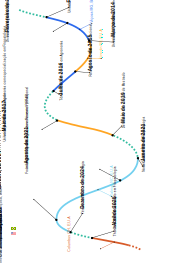
\includegraphics[width=\textwidth,height=0.8\textheight,keepaspectratio]{images/timeline.pdf}
  \end{center}
  \caption*{
    \textbf{Linha do tempo} (fora de escala) resumindo minha trajetória
    acadêmica, desde o início do meu curso de Bacharelado em Engenharia Agronômica na
    \UFV{} em 2011, até tempos atuais na \OSU{}.
  }
\end{figure}

%==============================================================================
\tableofcontents

\mainmatter
\pagestyle{fancy}

%==============================================================================
\chapter{Introdução}
\label{cap_intro}

\begin{figure}[h]
  \HeroFigPad
  \begin{center}
    \includegraphics[width=0.7\textwidth]{images/1994-soja.JPG}
  \end{center}
  \caption{
   Meu pai e eu, em visita às lavouras de soja em Viradouro, São Paulo. A foto foi tirada em 1994.
  }
  \label{fig_soja}
\end{figure}
\begin{summarybox}[frametitle=\faInfoCircle{}\quad Informações para contato]
  \begin{fa-ul}
    \faEnvelope & Email: \href{mailto:\Email}{\Email} \\
    \aiOrcid & ORCID: \href{https://orcid.org/\ORCID}{\ORCID} \\
    \aiLattes & Currículo Lattes: \url{https://lattes.cnpq.br/\Lattes} \\
    \faUser & Página pessoal: \url{https://agprophet.netlify.app/} \\
    \faLinkedin{} & LinkedIn: \href{https://www.linkedin.com/in/viniciusgarnica/}{viniciusgarnica} \\
    \faTwitter{} & Twitter: \href{https://twitter.com/agprophet_/}{@agprophet\_} \\
    \faUser & FFAR: \href{https://ffar.maps.arcgis.com/apps/Cascade/index.html?appid=89533a08df1a48b3a84df5a51ec5134c}{Vinicius Garnica} \\
  \end{fa-ul}
\end{summarybox}

Este memorial traça minha trajetória acadêmica e profissional, desde as raízes na agricultura familiar no interior
de São Paulo até minha atuação atual como pesquisador em epidemiologia vegetal. Mais do que um relato cronológico,
este texto propõe uma reflexão sobre como experiências vividas no campo e na academia moldaram minhas escolhas 
profissionais, consolidaram meu compromisso com a agricultura sustentável e alimentam minha visão para o futuro 
da fitopatologia digital.

\section{Influências durante a infância e a adolescência}

Meu primeiro contato com a ciência agronômica não se deu em salas de aula ou laboratórios, mas no cotidiano da 
propriedade rural de minha família, em Viradouro, interior de São Paulo. Filho de um agricultor e de 
uma professora da rede pública, cresci entre lavouras de soja, pomares de laranja e cultivos de cana de 
açúcar. Foi nesse ambiente que desenvolvi, ainda criança, uma compreensão prática dos desafios enfrentados 
no dia a dia pelo produtor rural. Lembro com nitidez das visitas que fazia aos talhões com meu pai (Figura~\ref{fig_soja}).

Em 2004, aos 12 anos, minha família vivenciou um episódio que marcou profundamente nossa relação com a 
agricultura: a chegada da ferrugem asiática da soja
(\href{https://en.wikipedia.org/wiki/Soybean_rust}{\textit{Phakopsora pachyrhizi}}) ao Brasil. A doença 
surgiu precocemente em nossas lavouras, e ninguém sabia ao certo o que fazer. Havia muita desinformação 
e incerteza. Aplicávamos tebuconazol com pulverizadores improvisados, sem saber se aquilo realmente resolvia o problema.

Pouco tempo depois, a podridão vermelha da raiz da soja
(\href{https://en.wikipedia.org/wiki/Sudden_death_syndrome}{\textit{Fusarium} spp.}) também atingiu 
nossas plantações em Minas Gerais. Eu ainda não compreendia as causas desses problemas nem a dimensão do prejuízo, 
mas nunca me esqueci de ver meu pai dirigir por mais de três horas até Jaboticabal, São Paulo, em busca de 
um parecer técnico no Laboratório de Diagnose de Solo, Planta e Fisiologia Vegetal da Universidade Estadual 
Paulista. O que eu não sabia em termos técnicos, já entendia em termos práticos: o custo da falta de informação.

Essas vivências me marcaram por presenciar de perto o impacto das doenças de plantas na vida das pessoas. Foi 
nesse contexto, ainda de forma intuitiva, que provavelmente nasceu meu interesse por fitopatologia. 
Um desejo de entender como as doenças interferem nas decisões agronômicas e de contribuir com soluções 
que tornem esse convívio mais previsível.

Além disso, com minha mãe, professora, e meu pai, agricultor, aprendi que ética, dedicação e conhecimento
caminham juntos. Essa base moldou a forma que penso e trabalho.

%==============================================================================
\chapter{Formação Acadêmica}
\label{cap_formacao}

\begin{figure}[h]
  \HeroFigPad
  \begin{center}
    \includegraphics[height=0.4\textheight, keepaspectratio]{images/2018-fungal-booth.jpg}
  \end{center}
  \caption{
  Momento de interação com estudantes de áreas correlatas. Um dos meus objetivos é ampliar o alcance 
  da fitopatologia, aproximando-a também de públicos diversos. No Brasil, onde a agricultura ainda 
  ocupa papel central, essa aproximação pode parecer menos urgente. No entanto, em países como os 
  Estados Unidos, onde cada vez menos pessoas estão diretamente ligadas à agricultura, a desconexão 
  entre ciência, produção agrícola e sociedade já é evidente. Precisamos nos preparar para essa 
  transição também no contexto brasileiro. A foto foi tirada durante a feira de ciências da \UNL{}, em 2018.
  }
\end{figure}
\begin{summarybox}[frametitle=\faInfoCircle{}\quad Resumo da formação acadêmica]
  \begin{datelist}
    2011--2016 & Bacharelado em Engenharia Agronômica --- \UFV{} \\
    2017--2019 & Mestrado em Agronomia com especialização em Fitopatologia --- \UNL{} \\
    2021--2024 & Ph.D. em Fitopatologia --- \NCState{}
  \end{datelist}
  \hrule
  \begin{datelist}
    2014--2015 & Intercâmbio internacional --- \UNL{} \\
    2025--atual & Pós-doutorado em Fitopatologia --- \OSU
  \end{datelist}
\end{summarybox}

Este capítulo apresenta minha trajetória de formação acadêmica, do bacharelado ao Ph.D., 
com reflexões sobre os fatores que influenciaram a definição das minhas linhas de pesquisa 
e o direcionamento da carreira profissional.

\section{\UFV{}}
\label{sec_ufv}

\begin{subsummarybox}[frametitle=\faGraduationCap{}\quad Bacharelado em Engenharia Agronômica]
  \begin{fa-ul}
    \faUniversity & \UFV{} \\
    \faCalendar & Fevereiro 2011 -- Julho 2016 \\
    \faUser & Orientadora: Dr. Leandro Grassi de Freitas\\
    \faInfoCircle & Trabalho de conclusão: Efeito da aplicação foliar de acefato e azadiractina na dinâmica 
    populacional do nematoide de cisto da soja (\textit{Heterodera glycines} Ichinohe)
  \end{fa-ul}
\end{subsummarybox}


Ingressei no curso de bacharelado em engenharia agronômica pela \UFV{} em 2011. Desde os primeiros semestres, 
o curso desafiou muitos dos conceitos que eu trazia da vivência com minha família no campo. Por sempre ter 
estado envolvido nas atividades da propriedade rural e auxiliado meu pai, minha compreensão da agricultura 
era bastante homogênea. A graduação expandiu minha base científica e atribuiu fundamentos técnicos a diversas 
práticas de cultivo que adotávamos de forma empírica.

Ciência do solo foi uma das áreas que mais despertaram meu interesse ao longo da graduação (e entomologia e matologia, 
as que menos). Em uma atividade prática, mapeamos a compactação do solo em uma lavoura de milho utilizando 
um penetrômetro de impacto e uma malha amostral predefinida. Por meio da geoestatística, geramos mapas que 
indicavam onde a subsolagem era realmente necessária. Também estimamos os 
custos da subsolagem total em comparação à localizada, demonstrando seu potencial de economia. Essa 
experiência despertou meu interesse por modelagem geoespacial, semivariogramas e estatística espacial 
aplicada à agricultura. Estou explorando esses temas novamente durante meu 
pós-doutorado na \OSU{}.

\subsection{Iniciação científica}

No segundo ano da graduação, iniciei dois projetos de iniciação científica sob orientação do professor 
Luiz Antonio Maffia, no Laboratório de Controle Biológico e Epidemiologia da \UFV{}. Trabalhei com 
supervisão direta de estudantes de pós-graduação, entre eles a doutora Elisa Silvera Pérez e 
o \href{https://www.linkedin.com/in/wanderson-bucker-moraes-31b06434/}{Dr. Wanderson Bucker de Moraes}.

O primeiro projeto teve como objetivo investigar a sensibilidade de isolados de 
\href{https://en.wikipedia.org/wiki/Botrytis_cinerea}{\textit{Botrytis cinerea}} à 
fungicidas. Participei de todas as etapas experimentais, desde o preparo dos meios de cultura 
com ingredientes ativos até o isolamento do patógeno a partir de amostras de rosas infectadas. 
Os dados gerados contribuíram para a construção de curvas dose-resposta e para estimativas de 
inibição fúngica, sendo apresentados no 46º Congresso Brasileiro de Fitopatologia, realizado 
em Ouro Preto (MG), minha primeira participação em um evento científico \citep{Garnica2013}.

No segundo projeto, colaborei no estudo da distribuição espacial da morte súbita da mangueira, 
causada por \href{https://en.wikipedia.org/wiki/Ceratocystis_fimbriata}{\textit{Ceratocystis fimbriata}}. 
Doenças de plantas raramente apresentam distribuição espacial aleatória em condições naturais de 
infestação. A compreensão desses padrões espaciais pode revelar rotas de disseminação e subsidiar 
estratégias de manejo. Nesse trabalho de campo, realizamos expedições mensais às regiões de 
Frutal (MG) e Itaocara (RJ), coletando dados sobre severidade e localização de cancros. Os 
resultados foram apresentados no APS-CPS Joint Meeting de 2014 \citep{Bucker2014a,Bucker2014b,Bucker2014c}.

Essas experiências marcaram o início da minha formação prática em fitopatologia. Mais do que seguir protocolos, compreendi a importância
de quantificar padrões, interpretar variações espaciais e integrar evidências para gerar conhecimento 
aplicável. Foi nesse contexto que meu interesse por modelagem se intensificou, direcionando as
escolhas acadêmicas que fiz no mestrado e no doutorado.

\subsection{Intercâmbio internacional na \UNL{}}
\label{sec_inter}

\begin{subsummarybox}[frametitle=\faPlane{}\quad Intercâmbio internacional]
\begin{fa-ul}
\faUniversity & \UNL{}\\
\faCalendar & Abril 2014 -- Agosto 2015
\end{fa-ul}
\end{subsummarybox}

Desde o início da graduação na \UFV{}, cultivava o desejo de participar de um intercâmbio internacional. Com 
frequência, acompanhava as oportunidades divulgadas pela universidade, em busca de programas que 
complementassem minha formação em agronomia. Uma das instituições que mais me atraiu foi 
a \href{https://www.unl.edu/}{\UNL{}}, reconhecida por sua excelência em pesquisa agrícola.

O processo seletivo era altamente competitivo, com vagas limitadas para estudantes de todo o Brasil 
por meio do programa Ciência sem Fronteiras. Após meses de preparação e envio de documentação, fui 
selecionado e embarquei para Lincoln, Nebraska, em abril de 2014. Na época, eu mal conseguia dizer um 
simples How are you?. Entretanto, minha experiência na UNL superou todas as expectativas. Encontrei um ambiente extremamente acolhedor e uma estrutura de pesquisa de 
excelência. Tive a oportunidade de cursar disciplinas avançadas em fitopatologia, sensoriamento 
remoto e entomologia, complementando conteúdos que só seriam abordados nos últimos semestres da 
graduação no Brasil.

Um dos destaques dessa vivência foi o trabalho no laboratório do \href{https://plantpathology.unl.edu/person/loren-giesler/}{Dr. Loren Giesler}, 
especialista em doenças da soja. Suas orientações e a convivência no laboratório me proporcionaram uma 
base teórica e prática que seria fundamental para o mestrado. Durante esse período, desenvolvi meu primeiro 
projeto independente, no qual investiguei o efeito de inseticidas na dinâmica populacional do 
nematoide de cisto da soja \href{https://en.wikipedia.org/wiki/Soybean_cyst_nematode}{(\textit{Heterodera glycines})}. 
Esse trabalho foi apresentado na feira científica de estudantes de graduação da UNL e conquistou o 
primeiro lugar na competição.

Além do crescimento acadêmico, meu tempo em Nebraska foi uma rica experiência cultural. Ao conviver 
com estudantes de diversas nacionalidades, ampliei minha visão de mundo e sobre mim mesmo.

Os conhecimentos adquiridos na UNL foram imediatamente aplicados ao meu trabalho de conclusão de
curso e abriram portas para o mestrado nos Estados Unidos, iniciando uma trajetória acadêmica 
internacional que segue até hoje.

\subsection{Reflexões}

Retornei ao Brasil em agosto de 2015, após cumprir o estágio obrigatório em uma empresa produtora de sementes de milho híbrido 
em Nebraska. Hoje, olhando para trás, reconheço que minha trajetória na UFV foi marcada por intenso
desenvolvimento pessoal e profissional. Conquistei amizades duradouras e, ao longo de cinco anos e meio 
de curso (2011–2016, com extensão decorrente do intercâmbio), concluí 209 créditos em 58 disciplinas, 
totalizando 3.195 horas, conforme exigido para a graduação em engenharia agronômica.

Finalizei o curso com um trabalho de conclusão orientado pelo professor Dr. Leandro Grassi de Freitas, intitulado: 
  Efeito da aplicação foliar de acefato e azadiractina na dinâmica populacional do nematoide de cisto da 
soja (\textit{Heterodera glycines} Ichinohe).

O currículo abrangente da UFV proporcionou uma base sólida em todas as áreas da agronomia, com ênfase na 
formação em ciências básicas (biologia celular, química, cálculo), disciplinas técnicas essenciais
(topografia, meteorologia), e conhecimentos especializados (fitopatologia, entomologia agrícola, manejo 
                                                            de solos), além de componentes práticos (estágio supervisionado e trabalho de conclusão de curso). O 
intercâmbio na UNL, registrado como mobilidade acadêmica no histórico escolar, complementou essa 
formação com uma perspectiva internacional. Após vivenciar outras instituições de renome no exterior, 
reconheço ainda mais a importância de oferecer cursos de graduação de alta qualidade para formar 
profissionais preparados para os desafios contemporâneos. Por isso, sou profundamente grato a 
todos os professores e ao país, que me proporcionaram acesso a uma educação pública e transformadora. Muito obrigado!
  
  
\section{\UNL{}}
\label{sec_unl}

\begin{subsummarybox}[frametitle=\faGraduationCap{}\quad Mestrado em Agronomia e especialização em Fitopatologia]
\begin{fa-ul}
\faUniversity & \UNL{} \\
\faCalendar & Maio 2017 -- Maio 2019 \\
\faUser & Orientador: Dr. Loren Giesler \\
\faInfoCircle & Tese: Integrated management of Phytophthora stem and root rot of
soybean and the effect of soil-applied herbicides on seedling disease incidence
(\href{https://digitalcommons.unl.edu/agronhortdiss/161/}{Link})
\end{fa-ul}
\end{subsummarybox}

Após a graduação, iniciei minha carreira como trainee em uma empresa de sementes de soja no Mato Grosso, onde vivi de perto 
os desafios da agricultura em larga escala. Embora fora do meio acadêmico, essa experiência ampliou minha visão sobre o 
que realmente importa no campo. Um ano depois, em maio de 2017, retornei aos Estados Unidos para iniciar o mestrado na \UNL{}.

Durante o mestrado, aprofundei meus conhecimentos em Fitopatologia por meio de disciplinas avançadas. Paralelamente, concentrei grande parte dos 
créditos em métodos estatísticos, obtendo o título de mestre com minor em estatística. Em disciplinas como STAT 801 (Statistical Methods in Research) e STAT 802 (Design and Analysis of Research Studies), ministradas pelo \href{https://statistics.unl.edu/person/kent-m-eskridge/}{Dr. Kent Eskridge}, 
aprendi fundamentos da análise de experimentos controlados. Essa familiaridade com modelos estatísticos me 
permitiu não apenas analisar os dados coletados durante o mestrado, mas também compreender a lógica por trás da modelagem estatística. 
Em um trabalho posterior\footnote{\url{https://apsjournals.apsnet.org/doi/10.1094/PDIS-11-23-2519-SR}}, por exemplo, 
utilizei esse conhecimento para simular dados multiambientais de eficiência agronômica de fungicidas para testar e validar algorítimos estatísticos. 
De fato, essa base adquirida no mestrado tem sido fundamental para as análises que realizo até hoje.

\subsection{Pesquisa}

O foco da minha pesquisa de mestrado foi compreender os fatores associados à ocorrência de 
doenças de solo em plântulas e à podridão radicular da soja, com ênfase em \href{https://en.wikipedia.org/wiki/Phytophthora_sojae}{\textit{Phytophthora sojae}}, um dos principais 
patógenos da soja no Meio-Oeste dos Estados Unidos\footnote{Mais informações em \url{https://cropprotectionnetwork.org/publications/soybean-disease-loss-estimates-from-the-united-states-and-ontario-canada-2024}}.
Um aspecto particularmente relevante observado durante o estudo foi a grande variação interanual e entre ambientes na ocorrência e severidade dessas doenças, mesmo em áreas com histórico conhecido de incidência. 
Essa variação evidencia a complexa interação entre clima, hospedeiro, população de patógenos e as estratégias de manejo adotadas a cada safra.

Durante o mestrado, também conduzi um levatamento populacional de \textit{P. sojae} para avaliar a eficácia de 
genes de resistência específicos (\textit{Rps}) no estado. De 2016 a 2018, mais de 100 isolados foram coletados e caracterizados quanto 
à virulência em 15 genótipos diferenciadores de soja. Identificamos 15 patótipos em Iowa e 10 em Nebraska \citep{Matthiesen2021}. 
Participei ainda de uma meta-análise com 5.121 isolados de \textit{P. sojae} coletados entre 1990-2019 em 29 
levantamentos globais \citep{McCoy2023}. Decidi não aprofundar esses trabalhos da minha linha de pesquisa principal pois, embora tenham alto impacto,
são projetos secundários que conduzi e gostaria de focar nos pontos que me interesso mais no capítulo~\ref{cap_pesquisa}.

Assim como pretendo mostrar no capítulo~\ref{cap_pesquisa}, minha linha de pesquisa tem sido bastante diversificada mas sempre relacionada à 
interação entre clima, hospedeiro, patógeno no desenvolvimento de epidemias de plantas. Além disso, essas experiências diversas 
demonstraram minha capacidade de trabalhar em equipes multidisciplinares, habilidade que pretendo continuar desenvolvendo na \USP{}. Durante o mestrado, 
também tive a oportunidade de mentorar estudantes de graduação, ajudando-os a compreender conceitos complexos de Fitopatologia e estimulando o pensamento crítico.

\subsection{Agradecimentos}

Gostaria de registrar meu profundo agradecimento ao \href{https://agronomy.unl.edu/jhala/}{Dr. Amit Jhala}, à \href{https://directory.unl.edu/people/tjackson3}{Drª Tamra Jackson-Ziems}  e 
ao \href{https://plantpathology.unl.edu/person/robert-harveson/}{Dr. Robert Harveson} pelo apoio durante minha formação na University of Nebraska–Lincoln. Cada um,
à sua maneira, contribuiu para meu crescimento acadêmico e profissional nesse período fundamental da minha 
trajetória. Em especial, expresso minha sincera gratidão ao Loren. Sua confiança e generosidade 
abriram portas que, na época, eu não teria conseguido transpor sozinho. Loren me deu oportunidades 
de participar de projetos relevantes e me conectou a redes profissionais importantes. Mesmo após uma década desde nosso 
primeiro contato, ele continua sendo um mentor presente.

\section{\NCState{}}
\label{sec_ncstate}

\begin{subsummarybox}[frametitle=\faGraduationCap{}\quad Ph.D. em Fitopatologia]
\begin{fa-ul}
\faUniversity & \NCState{} \\
\faCalendar & Janeiro 2021 -- Dezembro 2024 \\
\faUser & Orientador: Dr. Peter Ojiambo \\
\faInfoCircle & Dissertação: Influence of environment, risk of disease occurrence and cultivar 
stability to Stagonospora nodorum blotch in winter wheat (\href{https://repository.lib.ncsu.edu/items/008c6b45-149b-4932-a2f3-ef03b498dd05}{Link}) \\
\faYoutube & Vídeo sobre o projeto de pesquisa: \url{https://www.youtube.com/watch?v=8acqdIwAOHw}
\end{fa-ul}
\end{subsummarybox}

A epidemiologia vegetal sempre foi a área da fitopatologia que mais me interessou. Há algo profundamente 
satisfatório em transformar a complexidade biológica em modelos que explicam e, em certos casos, antecipam 
o comportamento das doenças. No doutorado, mergulhei nesse desafio: desenvolver modelos que não apenas 
descrevessem epidemias, mas que fossem úteis, capazes de informar decisões práticas no campo.

Antes de entrar nos detalhes, quero explicar de forma simples como entendo a modelagem matemática em 
sistemas biológicos. Talvez outros pesquisadores tenham visões diferentes, mas, para mim, modelar é 
uma tentativa de traduzir a realidade, muitas vezes desorganizada e cheia de ruído, em algo que possamos 
compreender, analisar, reproduzir e, em algumas situações, prever. É simplificar sem perder o essencial. 
É reduzir milhares de observações a poucos parâmetros que, combinados, fazem sentido. Essa busca exige 
clareza de pensamento para responder perguntas fundamentais: o que realmente está acontecendo neste 
sistema? Quais variáveis são relevantes? Como elas se relacionam? Quando usamos dados para 
responder a essas perguntas, deixamos de apenas descrever e passamos a explicar e antecipar. 

Essa busca por clareza conceitual me levou à estatística 
Bayesiana\footnote{Mergulhei na estatística Bayesiana após ser selecionado e participar 
  de um curso na Colorado State University em 2023: \url{https://www.nrel.colostate.edu/projects/bayesian/}.}. O 
paradigma Bayesiano se destaca na epidemiologia vegetal por permitir a incorporação de conhecimento 
prévio e a construção de modelos hierárquicos e flexíveis. Essas são características essenciais para lidar com dados 
epidemiológicos. Esse interesse também me abriu portas para o desenvolvimento em programação, 
software livre e ciência aberta. Embora já utilizasse \texttt{R}\footnote{Mais informações 
  disponíveis em: \url{https://www.r-project.org/}} desde 2017, passei a adotar controle de v
ersão com Git, publicar repositórios no GitHub e construir páginas web, habilidades que hoje considero 
centrais para uma formação superior mais integrada e atual em ciências agrárias.

Minha pesquisa de doutorado teve como foco a mancha de Stagonospora do trigo
(\href{https://en.wikipedia.org/wiki/Phaeosphaeria_nodorum}{\textit{Stagonospora nodorum}}). Na Carolina 
do Norte, onde cerca de 200 mil hectares de trigo são cultivados anualmente, essa doença pode causar 
perdas de até 30 por cento. O manejo envolve uma combinação de cultivares resistentes, manejo de 
palhada e aplicação de fungicidas. Entretanto, como a ocorrência da doença é esporádica e ainda 
faltam ferramentas digitais de apoio à decisão, muitos produtores seguem calendários fixos de 
pulverização, sem avaliar se as condições realmente exigem a aplicação.

Diante desse cenário, meu orientador, \href{https://cals.ncsu.edu/entomology-and-plant-pathology/people/pojiamb/}{Dr. Peter Ojiambo}, e 
eu definimos o objetivo central do doutorado: desenvolver uma abordagem preditiva que ajudasse a antecipar 
o risco de ocorrência da doença com base na tríade hospedeiro, patógeno e ambiente. Os principais eixos da 
pesquisa incluíram:
  
\begin{itemize}
  \item Customização de variáveis climáticas (temperatura, umidade e precipitação) associadas à mancha de Stagonospora, com alta resolução temporal
  \item Avaliação da estabilidade de cultivares resistentes em ensaios multiambientais
  \item Modelagem quantitativa, probabilística e aprendizado de máquina
  \item Quantificação das perdas causadas pela doença e a avaliação de diferentes níveis de entrada no sistema de manejo
\end{itemize}

O objetivo final foi desenvolver a base técnica para um sistema de alerta precoce, que permitisse 
substituir o manejo calendarizado por decisões baseadas no risco real de epidemia.

\subsection{Conquistas}

Durante o doutorado, fui selecionado para apresentar meu trabalho no
\href{https://www.apsnet.org/members/give-awards/foundation/awardees/Pages/2024.aspx}{I. E. Melhus Graduate Student Symposium}, 
realizado durante o congresso Plant Health 2024, em Memphis, Tennessee. Trata-se de uma das sessões muito prestigiadas do 
evento internacional promovido pela American Phytopathological Society. A seleção é altamente competitiva e reconhece os 
melhores trabalhos desenvolvidos por doutorandos em Fitopatologia. Até hoje, poucos brasileiros participaram dessa sessão,
o que torna essa conquista ainda mais significativa. Sou especialmente grato ao meu orientador pelos direcionamentos 
que possibilitaram essa realização.

Também fui agraciado com o \textit{Professional Development Award}, concedido pelo Departamento de Entomologia e 
Fitopatologia da \NCState{}, em reconhecimento ao desempenho acadêmico e à contribuição científica ao 
departamento. Além disso, integrei uma equipe interdisciplinar de estudantes de diferentes departamentos que conquistou o segundo lugar no
\href{https://cals.ncsu.edu/psi/news/third-annual-n-c-psi-hackathon-brings-in-record-numbers/}{Advanced Machine Learning Hackathon}, 
promovido pela NC State. Na ocasião, desenvolvemos modelos preditivos com base em dados agronômicos, o que 
reforçou minha capacidade de integrar ciência de dados e agricultura, com foco em abordagens estatísticas interpretáveis.

\subsection{Programa de desenvolvimento profissional}

Poderia omitir esta parte, mas seria injusto. O programa \href{https://ffarfellows.org/}{Rockey FFAR Fellows} teve um 
impacto profundo na minha formação. Em um sistema que frequentemente valoriza exclusivamente a produção técnica, 
esse programa mostrou que saber liderar, servir, comunicar, colaborar
e conhecer a si mesmo é tão ou mais importante do que publicar um artigo científico.

\begin{figure}[h]
\HeroFigPad
\begin{center}
  \includegraphics[height=0.4\textheight, keepaspectratio]{images/ffar_2023.jpg}
\end{center}
  \caption{
    As sessões presenciais com estudantes do FFAR foram momentos de grande crescimento pessoal e profissional. Participamos de 
    treinamentos em oratória, comunicação científica e autoconhecimento, além de cultivar amizades duradouras. A foto mostra 
    participantes de diferentes edições do FFAR, tirada nas proximidades da \NCState{} em 2023.
  }
  \label{fig_ffar}
\end{figure}
  
O programa oferece um treinamento profissional singular por meio de oficinas de aprendizado e encontros anuais que ampliaram meu autoconhecimento.
Além disso, conviver com bolsistas de diferentes origens e formações expandiu minha rede de contatos e minha visão de mundo.
A diversidade de trajetórias e formas de pensar me ensinou a escutar com mais atenção e trabalhar em equipe (Figura~\ref{fig_ffar}).

Sou grato à Dra. Rebecca Dunning, aos mentores envolvidos, à FFAR e à United Phosphorus Limited — esta última 
e a FFAR pelo financiamento dessa experiência. Muito obrigado!
    
    
\subsection{Reflexões}

Finalizo este capítulo com uma reflexão importante: embora dedicação, esforço e talento certamente 
tenham contribuído para meu percurso profissional, seria ingênuo atribuir toda a minha trajetória 
apenas ao mérito pessoal. Muitos outros fatores, estruturais, históricos e pessoais, também me 
favoreceram. Reconhecer isso não diminui meu esforço, mas reforça o papel que outros tiveram na minha trajetória.

Sou profundamente grato aos professores do Departamento de Entomologia e Fitopatologia da
North Carolina State University, cujas contribuições técnicas foram fundamentais ao longo do meu doutorado. Destaco o
\href{https://cals.ncsu.edu/entomology-and-plant-pathology/people/macubeta/}{Dr. Marc Cubeta},
\href{https://cals.ncsu.edu/entomology-and-plant-pathology/people/drotenb/}{Dr. Dorith Rotenberg} e
\href{https://phylodynamics.wordpress.ncsu.edu/people/david-rasmussen/}{Dr. David Rasmussen},
que ajudaram meu programa de estudos direta ou indiretamente.

Do Departamento de Estatística, agradeço especialmente ao
\href{https://statistics.sciences.ncsu.edu/people/jaosborn/}{Dr. Jason Osborne}, cujo rigor
metodológico consolidou minha base teórica, inclusive nas três vezes em que me questionou, durante o 
exame de qualificação, sobre a diferenciação entre erro do tipo I e erro do tipo II. Registro também,
minha gratidão ao \href{https://statistics.sciences.ncsu.edu/people/boos/}{Dr. Dennis Boos}, sempre 
generoso com seu tempo para conversas sobre estatística, vida acadêmica e as diferenças 
culturais entre Brasil e Estados Unidos.

Na área de extensão, sou grato à \href{https://www.ces.ncsu.edu/profile/angela-post/}{Dra. Angela Post},
pela parceria em ensaios de campo e pelos ensinamentos sobre a cultura do trigo, uma realidade que, até então, eu conhecia apenas pela televisão.

Outros pesquisadores exerceram grande influência na minha formação. O \href{https://www.linkedin.com/in/denis-shah-28360120}{Dr. Denis Shah}
foi uma presença constante e generosa, com quem mantive longas conversas sobre pensamento
epidemiológico e sobre a tradução de hipóteses biológicas em modelos analíticos. Já o
\href{https://plantpath.psu.edu/directory/pde6}{Dr. Paul Esker},
junto com meu orientador, liderou os projetos que financiaram meu doutorado. Com ambos aprendi não 
apenas ciência, mas também a conduzir pesquisas com relevância prática e propósito claro. Tive meus estudos 
integralmente financiados por projetos que eles escreveram e, graças a isso, pude desenvolver algumas pesquisas de descrevo abaixo.

Também contribuíram tecnicamente com meus projetos o
\href{https://www.lsu.edu/agriculture/ppcp/people/profile/felipe-dalla-lana.php}{Dr. Felipe Dalla Lana},
\href{https://www.linkedin.com/in/olanrewaju-shittu-m/}{Olanrewaju Shittu}
e o melhorista de plantas
\href{https://scholar.google.com/citations?user=kHw-7L4AAAAJ&hl=en}{Dr. Mohammad Nasir Shalizi},
cujo conhecimento aplicado enriqueceu diversas etapas da minha pesquisa.
  
\section{\OSU{}}
\label{sec_OSU}
  
\begin{subsummarybox}[frametitle=\faGraduationCap{}\quad Pós-doutorado em Fitopatologia]
  \begin{fa-ul}
  \faUniversity & \OSU{} \\
  \faCalendar & Abril 2025 -- Presente \\
  \faUser & Orientador: Dr. Horacio Nicora-Lopez \\
\end{fa-ul}
\end{subsummarybox}
  
Atualmente, atuo como pesquisador de pós-doutorado no Departamento de Fitopatologia da \OSU{}, em colaboração com o
\href{https://plantpath.osu.edu/our-people/horacio-lopez-nicora}{Dr. Horacio Lopez-Nicora}. Minhas atividades 
concentram-se em epidemiologia vegetal, com ênfase em análise estatística aplicada às doenças da soja, 
especialmente o nematoide de cisto da soja e doenças foliares.

Apesar do curto período desde o início dessa etapa, venho desenvolvendo atribuições em diferentes frentes:
    
\begin{itemize}
 \item Condução de meta-análises, tanto frequentistas quanto Bayesianas, sobre a eficácia de tratamentos de sementes e fungicidas foliares
 \item Desenvolvimento e aplicação de modelos espaciais para descrever padrões de ocorrência e severidade de patógenos da soja no estado de Ohio
 \item Padronização de fluxos analíticos, integrando práticas de ciência aberta, como controle de versão via GitHub, uso de plataformas de preprints e repositórios públicos de dados
 \item Preparação de manuscritos científicos interdisciplinares voltados à epidemiologia vegetal
 \item Orientação de estudantes de graduação e pós-graduação em atividades de pesquisa, incluindo análise de dados, condução de experimentos e comunicação científica
\end{itemize}
  
Esse trabalho tem aprofundado minha formação em estatística e fortalecido minha atuação no desenvolvimento de ferramentas computacionais aplicadas à Fitopatologia quantitativa.


%==============================================================================
\chapter{Linhas de Pesquisa}
\label{cap_pesquisa}
  
\begin{figure}[h]
\HeroFigPad
\begin{center}
  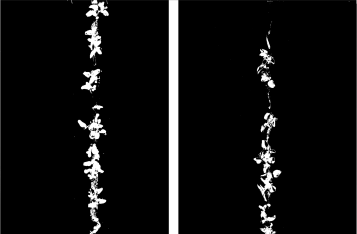
\includegraphics[width=\textwidth]{images/canopy.jpg}
  \end{center}
  \caption{
    Comparação do desenvolvimento do dossel da soja em plântulas com e sem tratamento de semente, 
    sob condições de alto inóculo de patógenos de solo, conforme publicado em \citet{Garnica2019}.}
  \label{fig_dossel}
  \end{figure}
  
  
\begin{subsummarybox}[frametitle=\faInfoCircle{}\quad Resumo das atividades]
\begin{fa-ul}
  \faFilePdf & 5 artigos publicados em revistas, 2 artigos científicos em revisão, 
  6 artigos científicos em preparo, 15 trabalhos em anais de eventos \\
  \faComment & 9 apresentações de trabalho, sendo 2 dessas convidadas\footnotemark[1] \\
  \aiGoogleScholarSquare & 58 citações no Google Scholar (acesso em 2025-07-29)\\
  \end{fa-ul}
  \end{subsummarybox}
  \footnotetext[1]{O número de total trabalhos e apresentações pode ser diferente
    das quantidades listadas acima. Alguns trabalhos e apresentações estão
    listados em outras áreas de atuação ou
    pertencem a mais de uma linha de pesquisa.}
  
Ao longo da minha breve trajetória como pesquisador, procurei 
direcionar meus estudos para temas que permitissem integrar minha formação em Engenharia Agronômica, Fitopatologia e 
Estatística. Acredito que a convergência entre biologia aplicada e ferramentas computacionais representa um 
caminho promissor para gerar conhecimento útil à tomada de decisão na agricultura. Em geral, acredito que 
meus trabalhos, que vêm sendo bem citados\footnote{Segundo análise das plataformas Dimensions e Altmetric. Por exemplo:
\url{https://badge.dimensions.ai/details/id/pub.1121309431} \citep{Garnica2019},
\url{https://badge.dimensions.ai/details/id/pub.1139765506} \citep{Matthiesen2021} e
\url{https://nature.altmetric.com/details/154725903} \citep{McCoy2023}.}.

Este capítulo apresenta uma síntese das principais linhas de pesquisa que venho desenvolvendo, 
organizadas de acordo com minha afinidade temática e intenção de continuidade no futuro. Embora 
várias publicações ainda estejam em processo de revisão ou em fase de elaboração, o objetivo aqui 
é evidenciar os eixos de investigação que pretendo aprofundar como pesquisador independente.
  
\section{Modelos quantitativos para predição de epidemias de doenças de plantas}
\label{sec_modelagem}
  
\begin{summarybox}[frametitle=\faInfoCircle{}\quad Resumo da linha de pesquisa]
\begin{fa-ul}
  \faFilePdf & 2 artigos em preparo \\
  \faComment & 3 apresentações de trabalho \\
\end{fa-ul}
\end{summarybox}
  
\begin{subsummarybox}[frametitle=\faFilePdf{}\quad Artigos em preparo]
\begin{paperlist}
  202x & \Me, \Peter.
  Predicting Stagonospora nodorum blotch in winter wheat using a Bayesian hierarchical approach.
  Para ser submetido ao jornal \emph{Ecological Applications}.
  \\
  202x & \Me, \Angela, \Peter.
  Advancing Stagonospora nodorum blotch management in South Atlantic U.S. wheat with 
  uncertainty-aware model validation, yield loss quantification, and risk-based fungicide thresholds.
  Para ser submetido ao jornal \emph{Plant Disease}.
  \\
\end{paperlist}
\end{subsummarybox}
\begin{subsummarybox}[frametitle=\faComment{}\quad Apresentações]
\begin{paperlist}
  2024 & \Me.
  Novel approaches for plant disease prediction: a case with Stagonospora nodorum
  blotch of wheat. \emph{Annual Meeting of the Georgia Association of Plant Pathologists}, 
  Mar 6, 2024, Savannah, GA, E.U.A. (Apresentação oral)
  \\
  2024 & \Me.
  Risk assessment models for improved fungicide decisions in winter wheat and a digital tool to 
  improve quantitative synthesis of agricultural research. \emph{Plant Health 2024}, 
  Jul 27–30, 2024, Memphis, TN, E.U.A. (Apresentação oral)
  \\
  2021 & \Cucak, \Felipe, \Lanre, \Me, \Peter, \Erick, \Denis, \Paul, \Esker.
  Development and integration of the new-age decision support in crop disease protection.
  \emph{2021 APS Annual Meeting Research On-Demand}.
  \\
\end{paperlist}
\end{subsummarybox}
  
A Fitopatologia se apoia na observação e na experimentação como bases fundamentais. No entanto, a dinâmica das 
epidemias, moldada por interações entre patógeno, hospedeiro, ambiente e manejo, exige mais do que descrição empírica. 
Nesse contexto, a modelagem quantitativa torna-se essencial, organizando dados e formalizando hipóteses
para lidar com essa complexidade.

Mais do que estimar o risco, é preciso compreender também o grau de confiança nas previsões. Modelos 
probabilísticos que quantificam incertezas oferecem suporte mais robusto à tomada de decisão, 
sobretudo diante da variabilidade natural dos sistemas epidemiológicos. Sem essa abordagem, a 
previsão de doenças permanece limitada como ferramenta de manejo.

Durante o doutorado em Fitopatologia na \NCState{} (seção~\ref{sec_ncstate}), aprofundei essa linha de 
pesquisa usando a mancha de Stagonospora no trigo como patossistema modelo. Com base no paradigma 
Bayesiano, desenvolvemos modelos preditivos que integraram dados climáticos de alta resolução, 
estruturas hierárquicas para capturar variações espaciais e informações sobre o hospedeiro. Essa 
abordagem permite estimar a severidade da doença no campo e, ao mesmo tempo, quantificar a 
incerteza das previsões. Isso é um fator decisivo para recomendar, por exemplo, o momento mais adequado para aplicação de fungicidas.

As principais ferramentas utilizadas foram os pacotes
\texttt{brms}\footnote{\url{https://cran.r-project.org/web/packages/brms/index.html}}, que ajusta modelos
Bayesianos via \texttt{Stan}\footnote{\url{https://mc-stan.org/}}, e
\texttt{marginaleffects}\footnote{\url{https://cran.r-project.org/web/packages/marginaleffects/index.html}}, que facilita a 
interpretação e visualização de efeitos marginais.

Dois manuscritos estão em fase final de redação, acompanhados por um conjunto de códigos em \texttt{R} que será 
publicado como software livre. A ideia é que esses modelos possam ser utilizados, adaptados e 
aprimorados por outros pesquisadores, fortalecendo uma cultura científica mais colaborativa e aplicada.

Nos próximos anos, pretendo expandir essa linha de pesquisa em colaboração com grupos da USP, 
com foco na modelagem epidemiológica aplicada à Fitopatologia e no desenvolvimento de sistemas de 
apoio à decisão. A proposta inclui a criação de modelos e plataformas com previsões probabilísticas 
que orientem decisões práticas no campo. A USP oferece um ambiente fértil para esse tipo de iniciativa, 
ao exemplo do sistema TempoCampo\footnote{\url{https://site.tempocampo.org/}}. Essa 
linha de pesquisa representa um passo importante para transformar o manejo de doenças em sistemas agrícolas mais 
sustentáveis no Brasil, integrando previsão, variabilidade ambiental e decisões guiadas por dados.
  
\begin{fancyenum}{\faBullseye}{Objetivos}
\item Aprimorar sistemas de alerta e monitoramento de doenças usando modelos quantitativos e probabilísticos de predição 
  de epidemias de doenças de plantas
 \item Disponibilizar ferramentas abertas, reprodutíveis e acessíveis para apoiar decisões agronômicas sob incerteza
\end{fancyenum}
  
\begin{fancyenum}{\faLightbulb}{Principais contribuições}
 \item Revisitação do arcabouço Bayesiano e hierárquico para previsão da mancha de Stagonospora em trigo
 \item Desenvolvimento de uma estrutura flexível, aplicável a diferentes patossistemas e contextos de manejo
\end{fancyenum}
\begin{fancyenum}{\faRocket}{Impacto da pesquisa}
 \item Trabalho pioneiro na aplicação de modelos Bayesianos quantitativos para previsão de doenças de plantas
\end{fancyenum}
  
  
  
\section{Variáveis climáticas para modelagem de doenças de plantas}
\label{sec_window}
  
\begin{summarybox}[frametitle=\faInfoCircle{}\quad Resumo da linha de pesquisa]
\begin{fa-ul}
 \faFilePdf & 1 artigo em revisão \\
  \faComment & 2 apresentações de trabalho \\
  \end{fa-ul}
\end{summarybox}
\begin{subsummarybox}[frametitle=\faFilePdf{}\quad Artigos em preparo]
\begin{paperlist}
  202x & \Me, \Peter.
  Leveraging window-pane analysis with environmental loadings of genotype-by-environment
  interaction to identify high-resolution weather-based variables associated with plant disease.  
  Em revisão no jornal \emph{Frontiers in Plant Science}.
\end{paperlist}
\end{subsummarybox}
\begin{subsummarybox}[frametitle=\faComment{}\quad Apresentações]
\begin{paperlist}
  2024 & \Me.
  Novel approaches for plant disease prediction: a case with Stagonospora nodorum
  blotch of wheat. \emph{Annual Meeting of the Georgia Association of Plant Pathologists}, 
  Mar 6, 2024, Savannah, GA, E.U.A. (Apresentação oral)
  \\
  2024 & \Me.
  Novel weather variables associated with epidemics of Stagonospora nodorum blotch
  of winter wheat.\emph{13\textsuperscript{th} International 
    Epidemiology Workshop}, Foz do Iguaçu, Brasil. (Apresentação oral)
  \\
\end{paperlist}
\end{subsummarybox}


Essa linha de pesquisa começou durante meu doutorado em Fitopatologia na \NCState{} (seção~\ref{sec_ncstate}) e 
tem se mostrado promissora para o avanço de sistemas de apoio à decisão no manejo de doenças e no uso mais eficiente de fungicidas.

Sabemos que variáveis climáticas como temperatura, umidade e precipitação influenciam diretamente o 
desenvolvimento das epidemias. Ainda assim, dois desafios permanecem: primeiro, como gerar preditores 
climáticos que de fato representem os processos biológicos envolvidos; segundo, como incorporar as 
interações entre genótipo e ambiente, reconhecendo que cultivares diferentes podem reagir de formas distintas às mesmas condições
ambientais.

Ao contrário das abordagens convencionais, que usam janelas fixas baseadas no calendário agrícola, 
aplicamos uma estratégia chamada análise de janelas temporais condicionadas à condutividade 
epidemiológica (\href{https://apsjournals.apsnet.org/doi/full/10.1094/PDIS-05-20-0952-RE}{\textit{window-pane analysis}}). Essa 
técnica permite explorar aspectos como a duração da exposição a condições críticas, a persistência dessas condições e o
momento do dia em que ocorrem, gerando variáveis climáticas que dialogam melhor com os mecanismos da doença. Nosso modelo 
de estudo foi a mancha de Stagonospora no trigo.

A motivação é simples. Resumir o clima por períodos arbitrários, como semanas ou meses, ignora o fato de que epidemias 
seguem o ambiente, não o calendário. Nossa abordagem busca identificar empiricamente padrões críticos, como “umidade 
relativa acima de 85 por cento por seis horas seguidas durante a noite, entre os dias trinta e quatro e quarenta e oito
antes do florescimento”, e incorporar essas informações em modelos preditivos mais realistas.

Embora essa técnica já tenha sido usada em alguns sistemas, sua aplicação para investigar como o ambiente influencia 
as respostas diferenciais entre cultivares é inédita em Fitopatologia.

Os primeiros algoritmos estão disponíveis em repositório público\footnote{\url{https://github.com/vcgarnica/SNB_window_pane}}, e 
gostaria de desenvolver uma plataforma automatizada que permitirá aplicar essa metodologia a diferentes culturas e doenças. A 
proposta é criar uma biblioteca de variáveis climáticas com alta resolução temporal, que possa servir de base para sistemas de 
alerta mais precisos e alinhados aos processos biológicos.

O primeiro artigo sobre esse trabalho está atualmente em revisão no periódico 
\href{https://www.frontiersin.org/journals/plant-science}{Frontiers in Plant Science}. Meu objetivo é expandir essa linha 
com meu grupo de pesquisa, unindo biologia e estatística para modelar epidemias e apoiar o manejo de doenças e servindo técnicas avançadas de
perfilagem ambiental ao melhoramento genético de plantas.

  
\begin{fancyenum}{\faBullseye}{Objetivos}
 \item Desenvolver variáveis climáticas de alta resolução alinhadas a mecanismos epidemiológicos
 \item Incorporar interações genótipo-ambiente em modelos empíricos de epidemias
\end{fancyenum}
  
\begin{fancyenum}{\faLightbulb}{Principais contribuições}
 \item Desenvolvimento de algoritmos abertos e reprodutíveis para extração de variáveis climáticas críticas
 \item Proposição de método robusto para minimizar falsos positivos na seleção de preditores
\end{fancyenum}
  
\begin{fancyenum}{\faRocket}{Impacto da pesquisa}
 \item Trabalho pioneiro com potencial para impactar fitopatologia, melhoramento genético e ecologia 
  ao explorar a interface entre perfilagem ambiental, genótipo-ambiente e modelagem epidemiológica
\end{fancyenum}
  
  

\section{Ferramentas livres e ciência aberta na Fitopatologia}
\label{sec_msefindr}

\begin{summarybox}[frametitle=\faInfoCircle{}\quad Resumo da linha de pesquisa]
\begin{fa-ul}
  \faFilePdf & 1 artigo publicado \\
  \faComment & 2 apresentações de trabalho \\
\end{fa-ul}
\end{summarybox}
\begin{subsummarybox}[frametitle=\faFilePdf{}\quad Artigos publicados ou em preparo]
\begin{paperlist}
  2024 & \Me, \Denis, \Esker, \Peter.
  MSE FindR: A Shiny \texttt{R} application to estimate mean square error using treatment means and post-hoc test results.
  \emph{Plant Disease},
  \DOI{10.1094/PDIS-11-23-2519-SR}.
  \GitHub{vcgarnica/MSE_FindR/}.
\end{paperlist}
\end{subsummarybox}
\begin{subsummarybox}[frametitle=\faComment{}\quad Apresentações]
\begin{paperlist}
  2022 & \Me, \Denis, \Esker, \Peter.
  MSE FindR: an R Shiny app tool for recovering variance in designed experiments using treatment means and post-hoc 
  test results. \emph{National FHB Forum}, Dez 4–6, 2022, Tampa, FL, E.U.A. (Poster)
  \\
  2022 & \Me, \Denis, \Esker, \Peter.
  Got Fisher's LSD or Tukey's HSD?: an R Shiny app tool for recovering variance in designed experiments when only mean and post-hoc tests are
  reported. \emph{2022 APS Annual Meeting}, Aug 6–10, 2022, Pittsburgh, PA, E.U.A. (Poster)
  \\
\end{paperlist}
\end{subsummarybox}

A ciência aberta tem redefinido os padrões da pesquisa científica: publicar resultados já não 
basta. É preciso tornar dados, códigos e métodos acessíveis e reproduzíveis. Na Fitopatologia, 
no entanto, a adoção plena desse paradigma ainda esbarra em barreiras técnicas e culturais. A falta
de padronização na divulgação de dados limita a reanálise de experimentos, enfraquece revisões 
sistemáticas e dificulta a construção de modelos preditivos robustos.

Foi diante desse cenário que desenvolvi o MSE FindR \citep{Garnica2024} durante meu Ph.D. na \NCState{} (seção~\ref{sec_ncstate}).
MSE FindR é uma aplicação em \texttt{R} Shiny que estima o erro quadrático médio (MSE) a partir de médias de tratamentos e 
agrupamentos post-hoc (como LSD ou Tukey), expandindo metodologias anteriores \citep{Ngugi2011}. 
A motivação surgiu da recorrente ausência de métricas
estatísticas básicas em relatórios técnicos, como os do \href{https://apsjournals.apsnet.org/page/php/pdmr}{Plant Disease Management Reports},
dificultando o reaproveitamento de estudos primários em metanálises.

Com o MSE FindR, esses dados podem ser resgatados de forma estatisticamente rigorosa, 
permitindo sua integração em sínteses quantitativas. A ferramenta é gratuita, aberta e 
acompanha documentação completa\footnote{\url{https://github.com/vcgarnica/MSE_FindR/}}. O artigo 
técnico foi publicado no periódico \emph{Plant Disease}, e a aplicação já é usada e citada por pesquisadores dentro e fora 
da área\footnote{\url{https://scholar.google.com/scholar?cites=4326618921649328146}}.

Mais do que uma ferramenta, o MSE FindR faz parte de uma linha de pesquisa voltada à
criação de soluções estatísticas abertas e aplicáveis à realidade da Fitopatologia. Pretendo consolidar 
esse esforço junto ao meu grupo de pesquisa.

\begin{fancyenum}{\faBullseye}{Objetivos}
  \item Desenvolver ferramentas de ciência aberta para Fitopatologia
\end{fancyenum}

\begin{fancyenum}{\faLightbulb}{Principais contribuições}
  \item Estimativa do MSE a partir de dados mínimos, viabilizando metanálises com estudos subnotificados
  \item Software livre e documentado para reuso por equipes técnicas e acadêmicas
\end{fancyenum}

\begin{fancyenum}{\faRocket}{Impacto da pesquisa}
  \item Primeira ferramenta livre em \texttt{R} voltada à reconstrução de variância a partir de resultados post-hoc.
  Abre caminho para uma Fitopatologia mais quantitativa e colaborativa.
\end{fancyenum}


\section{Eficácia de tratamentos de doenças de plantas em ensaios multilocais}
\label{sec_met}

\begin{summarybox}[frametitle=\faInfoCircle{}\quad Resumo da linha de pesquisa]
\begin{fa-ul}
  \faFilePdf & 2 artigos publicados \\
  \faFilePdf & 2 artigos em preparo\footnotemark[1] \\
  \faComment & 2 apresentações de trabalho \\
\end{fa-ul}
\end{summarybox}
\footnotetext[1]{Há outros artigos em elaboração, mas ainda em fases iniciais. Optei por não incluí-los neste momento.}

\begin{subsummarybox}[frametitle=\faFilePdf{}\quad Artigos publicados ou em preparo]
\begin{paperlist}
  202x & \Me, \Nasir, \Peter.
  Performance and stability of winter wheat cultivars to Stagonospora nodorum blotch epidemics in multi-environment trials.
  Em revisão no jornal \emph{Phytopathology}.
  \\
  202x & \Ali, \Fabiano, \Me, \Lindsey, \Horacio.
  Multi-environment evaluation of soybean cultivar resistance and fungicide profitability for managing Septoria brown spot in Ohio.
  Em preparo para ser submetido ao jornal \emph{Plant Disease}.
  \\
  2022 & \Me, \Amit, \Bob, \Loren.
  Impact assessment of residual soil applied pre-emergence herbicides on the incidence of soybean seedling diseases under field conditions.
  \emph{Crop Protection},
  \DOI{10.1016/j.cropro.2022.105987}.
  \\
  2019 & \Me, \Loren.
  Soybean canopy coverage, population, and yield responses to seed treatment and cultivar resistance to \textit{Phytophthora sojae} in Nebraska.
  \emph{Plant Health Progress},
  \DOI{10.1094/PHP-05-19-0036-RS}.
  \\
\end{paperlist}
\end{subsummarybox}
\begin{subsummarybox}[frametitle=\faComment{}\quad Apresentações]
\begin{paperlist}
  2024 & \Me, \Peter. 
  Stability of resistance to Stagonospora nodorum blotch in winter wheat cultivars evaluated in a multi-environmental study in North Carolina. 
  \emph{ ASA, CSSA, and SSSA International Annual Meetings}, Oct 29–Nov 1, St. Louis, MO, E.U.A. (Poster)
  \\
  2018 & \Me, Leef, N., \Loren Indeterminate cultivars and seed treatment effect on soybean yield components. 
  \emph{Nebraska Plant Breeding Symposium}, Mar 13, Lincoln, NE, E.U.A. (Poster)
  \\
\end{paperlist}
\end{subsummarybox}

Esta linha de pesquisa teve início durante meu mestrado na \UNL{} (seção~\ref{sec_unl}) e foi aprofundada durante
o Ph.D. em Fitopatologia na \NCState{} (seção~\ref{sec_ncstate}).

Um dos projetos investigou a estabilidade da resistência genética em cultivares de trigo frente à variabilidade ambiental. 
Fatores como inóculo, patótipos, clima e solo influenciam o progresso das epidemias e a avaliação da resistência 
em campo. Por isso, ensaios em múltiplos locais e safras são essenciais.

No entanto, mesmo cultivares previamente classificadas como resistentes podem apresentar respostas distintas sob 
diferentes condições ambientais. Assim, torna-se fundamental desenvolver métodos estatísticos que possibilitem
a análise robusta das interações genótipo-ambiente (G×A), com o objetivo de identificar materiais 
geneticamente estáveis e de amplo desempenho.

Nesse projeto, combinamos métricas epidemiológicas, como taxa de 
progresso da doença (estimadas a partir de modelos Gompertz, logístico, monomolecular), área sob a curva de progresso, 
severidade final e tempo até  50\% de incidência, com a modelos lineares mistos e 
técnicas multivariadas. O objetivo foi desmembrar os efeitos genotípicos e ambientais sobre 
a epidemia e melhorar a recomendação de ferramentas de manejo em cenários variados de produção.
Apesar de amplamente utilizados em melhoramento genético, esses métodos ainda são subexplorados na Fitopatologia. 
Seu potencial para qualificar a recomendação de cultivares e otimizar o uso de insumos como fungicidas é 
significativo. O manuscrito desse trabalho encontra-se em revisão no periódico \emph{Phytopathology}, e os códigos
utilizados estão disponíveis em na pasta do projeto no \href{https://github.com/vcgarnica/SNB_stability}{Github}.

A abordagem também foi aplicada à soja em dois projetos de controle integrado. Em um deles, usei modelos lineares para 
avaliar cultivares resistentes e tratamentos de sementes quanto à produtividade, estande e severidade. 
Um diferencial foi o uso de um aplicativo móvel para monitoramento do dossel, permitindo inferências mais
precisas sobre o impacto dos tratamentos em doenças radiculares e dossel da planta (Figura~\ref{fig_dossel}). 
Os resultados desse trabalho foram publicados no periódico \emph{Plant Health Progress} \citep{Garnica2019}, sendo esse
meu primeiro artigo como primeiro autor.

Pretendo expandir essa linha por meio da aplicação de modelos mistos lineares e não lineares em 
ensaios multilocais para melhorar inferências sobre tratamentos no manejo de doenças. 


\begin{fancyenum}{\faBullseye}{Objetivos}
\item Desenvolver métodos estatísticos para avaliação de ferramentas de controle de doenças, 
  com foco estabilidade de tratamentos sob variabilidade ambiental e climática
\end{fancyenum}

\begin{fancyenum}{\faLightbulb}{Principais contribuições}
  \item Aplicação de modelos mistos com estruturas de covariância 
  (e.g., fatorial, heterogeneidade residual) para modelar interações G×A em epidemias
  \item Disponibilização de algoritmos e códigos em software livre, promovendo reprodutibilidade e ciência aberta
\end{fancyenum}

\begin{fancyenum}{\faRocket}{Impacto da pesquisa}
  \item Fortalecimento da interface entre epidemiologia de campo e estatística aplicada,
  com ênfase em predição dos efeitos de tratamento sob variabilidade ambiental.
\end{fancyenum}



\section{Modelagem espacial para inferência da eficácia de tratamentos fitopatológicos}
\label{sec_spatial}

\begin{summarybox}[frametitle=\faInfoCircle{}\quad Resumo da linha de pesquisa]
\begin{fa-ul}
\faFilePdf & 1 artigos em preparo \\
\end{fa-ul}
\end{summarybox}
\begin{subsummarybox}[frametitle=\faFilePdf{}\quad Artigos em preparo]
\begin{paperlist}
  202x & \Me, \Horacio.
  Accounting for spatial trends improves the assessment of fluopyram and host resistance 
  efficacy against soybean cyst nematode in field trials.
  Em preparo para ser submetido ao jornal \emph{Phytopathology}.
\\
\end{paperlist}
\end{subsummarybox}

Apesar de poder ser incluída na seção~\ref{sec_met}, esta linha foi tratada separadamente por seu foco 
específico na estrutura espacial dos dados experimentais. Um dos principais desafios em ensaios de campo é o 
controle do ruído espacial, causado por gradientes de solo, umidade e infestação, que afetam 
diretamente as estimativas e podem mascarar efeitos reais.

Assim, durante meu pós-doutorado na \OSU{}, estou me aprofundando a aplicação de modelos com estrutura espacial para 
melhorar a inferência sobre o manejo do nematoide de cisto da soja. Apesar da reconhecida dependência espacial
desse patógeno, ainda há lacunas sobre como incorporar essa variabilidade na análise estatística.

Com dados de Ohio, testamos modelos residuais com dependência espacial, como AR1, P-splines e modelos com 
covariáveis ambientais (e.g., contagem de ovos), usando \texttt{ASReml-R}. Os resultados mostraram maior
precisão, menor erro residual e melhor distinção entre cultivares e tratamentos com modelos espaciais.

Esta linha busca consolidar a modelagem espacial como prática padrão na Fitopatologia, com aplicações 
tanto na inferência sobre tratamentos quanto na modelagem de epidemias.

\begin{fancyenum}{\faBullseye}{Objetivos}
\item Melhorar a inferência sobre eficácia de tratamentos para doenças de solo através de modelagem espacial
\end{fancyenum}

\begin{fancyenum}{\faLightbulb}{Principais contribuições}
\item Aplicação de modelos com covariáveis espaciais em experimentos com nematóide do cisto
\item Demonstração de melhoria substancial na detecção de diferenças entre tratamentos após ajuste espacial
\end{fancyenum}

\begin{fancyenum}{\faRocket}{Impacto da pesquisa}
\item Os métodos e ferramentas desenvolvidos têm potencial para uso em larga 
escala por programas de melhoramento, manejo integrado e pesquisa aplicada
\end{fancyenum}


%==============================================================================
  \chapter{Ensino}
\label{cap_ensino}

\begin{figure}[h]
\HeroFigPad
\begin{center}
\includegraphics[width=\textwidth]{images/cursoR.jpg}
\end{center}
\caption{
  O volume de dados na agricultura cresce continuamente, exigindo profissionais capacitados em 
  ferramentas analíticas modernas. Tenho contribuído com essa transição por meio de treinamentos 
  práticos em programação e do compartilhamento de códigos aplicados às ciências agrárias. A imagem 
  mostra um curso introdutório de \texttt{R} que ministrei com Daniela Cooney para pós-graduandos da \NCState{}.}
\label{fig_cursoR}
\end{figure}


\section{Monitor de aula no programa de pós graduação}
\begin{subsummarybox}[frametitle=\faFilePdf{}\quad Resumo das atividades]
\begin{datelist}
2023 & Monitor da disciplina PP506 – Epidemiologia e Controle de Doenças de Plantas, North Carolina State University \\
2022 & Monitor da disciplina PP506 – Epidemiologia e Controle de Doenças de Plantas, North Carolina State University
\end{datelist}
\end{subsummarybox}

Embora minha experiência formal em docência seja pontual, atuei por dois semestres como monitor da disciplina
de epidemiologia vegetal e manejo de doenças de 
plantas\footnote{PP506: Epidemiology and Plant Disease Control; \url{https://wolfware.ncsu.edu/courses/details/?sis_id=SIS:2022:1:1:PP:506:001}} 
na \NCState{}. Nessa função, ofereci suporte a estudantes de pós-graduação na assimilação de conceitos 
estatísticos e epidemiológicos aplicados à Fitopatologia.

A disciplina aborda fundamentos conceituais e quantitativos da epidemiologia vegetal, 
iniciando com aspectos históricos e terminológicos, passando pela mensuração 
de doenças e características do hospedeiro, e discutindo princípios de precisão, 
acurácia e estratégias de monitoramento. Ao longo do curso, os estudantes exploram 
a dinâmica temporal e espacial das epidemias por meio de modelos analíticos, 
incluindo Gompertz, monomolecular e exponencial, com ênfase na interpretação 
de curvas de progresso, avaliação de gradientes espaciais, análise de padrões 
de agregação e estimativas de perdas de produtividade.

\section{Atuação na comunidade científica}

\begin{subsummarybox}[frametitle=\faFilePdf{}\quad Resumo das atividades]
\begin{datelist}
2025 & Juiz na Feira Internacional de Ciências e Engenharia (ISEF), Columbus, Ohio \\
2023--2024 & Coordenador de seminários de comunicação científica, FFAR–NCSU \\
2022 & Instrutor do curso introdutório em R e estatística aplicada à ciências agrárias liderado por estudantes na \NCState{}
\end{datelist}
\end{subsummarybox}


Minha atuação na comunidade científica tem sido guiada pelo compromisso com a formação de 
pesquisadores em epidemiologia vegetal quantitativa, ciência reprodutível e comunicação 
científica. Ao longo dessa trajetória, treinei mais de 20 estudantes em \texttt{R} e ciência de 
dados com foco em aplicações práticas em agronomia e Fitopatologia.

\subsection{Seminários e oficinas}

Organizei e conduzi seminários mensais independentes focados no desenvolvimento de habilidades em comunicação científica 
entre estudantes de pós-graduação da NCSU, incluindo participantes do FFAR. Embora aberta a qualquer programa, a atividade 
não era oficialmente vinculada ao programa. Os encontros incluíam apresentações voluntárias de pesquisas em andamento ou 
ensaios de apresentações, seguidas por sessões de feedback entre pares. A iniciativa, liderada por mim, buscou aprimorar 
minhas habilidades de comunicação e, sobretudo, fortalecer minha capacidade de liderança e organização. Coordenei todas as 
etapas, desde a definição da agenda até a condução dos encontros e mediação das discussões. O formato informal, porém 
estruturado, incentivou a participação espontânea e criou um ambiente seguro para testar ideias e trocar críticas 
construtivas, beneficiando tanto quem apresentava quanto quem ouvia.

Também organizei e ministrei uma oficina técnica de análise de dados com \texttt{R} para a comunidade acadêmica da \NCState{},
como uma atividade liderada por nós, estudantes (Figura~\ref{fig_cursoR}). O curso, com dois dias de duração, abordou 
fundamentos do \texttt{R}, incluindo importação de dados, 
manipulação de tabelas, análises de variância e visualizações gráficas. O material didático está disponível 
em: \url{https://github.com/vcgarnica/NCSU_R_workshop_2022}.

\subsection{Atividades de revisão e julgamento técnico}

Embora tenha completado meu Ph.D. na NC State recentemente, tenho participado ativamente da comunidade 
científica, principalmente na interseção entre epidemiologia vegetal e ciência aberta. Também atuo como revisor de periódicos 
científicos\footnote{Mais informações disponíveis nos periódicos \textit{Plant Disease} e \textit{Tropical Plant Pathology}, 
ambos de destaque na área de Fitopatologia.}. Considerando que muitos excelentes cientistas 
brasileiros enfrentam barreiras com o inglês, pretendo utilizar minhas habilidades para 
capacitar estudantes de pós-graduação na prática da escrita científica em inglês.

Atuei também como juiz na Feira Internacional de Ciências e Engenharia (ISEF 2025)\footnote{\url{https://www.societyforscience.org/isef/}}, 
refletindo meu compromisso com o incentivo à ciência em estágios iniciais da carreira. Inclusive, 
me impressionei com a qualidade dos trabalhos conduzidos por estudantes tão jovens, alguns deles 
comparáveis ou superiores a projetos de doutorado. Também participei de bancas avaliadoras 
internas (e.g., comitê de contratação em 2018 na \UNL{}).


%==============================================================================
  \chapter{Extensão}
\label{cap_extensao}

\begin{figure}[h]
\HeroFigPad
\begin{center}
\includegraphics[width=\textwidth]{images/extensao.jpg}
\end{center}
\caption{
  Crescer no meio rural me ensinou a valorizar a agricultura e o trabalho daqueles que atuam diretamente no 
  campo. Por isso, decidi dedicar-me a servi-los por meio da Fitopatologia. A foto mostra uma 
  apresentação ténica que realizei sobre doenças da soja, em parceria com o programa de extensão 
  da \NCState{} no condado de Robeson em 2023.}
\label{fig_extensao}
\end{figure}



\begin{subsummarybox}[frametitle=\faFilePdf{}\quad Resumo das atividades]
\begin{datelist}
2024 & Palestrante no dia de campo para estudantes Latinos, Raleigh, Carolina do Norte \\
2023 &  Palestrante no encontro de milho e soja dos condados de Hoke–Robeson–Scotland na Carolina do Norte\\
2022 &  Identificação e monitoramento de doenças da soja. Dia de campo da soja na Estação de Pesquisa do Piedmont, Carolina do Norte
\end{datelist}
\end{subsummarybox}


Extensão, para mim, é levar a ciência de volta às pessoas. Crescer no meio rural me mostrou que o conhecimento técnico, 
quando bem comunicado, transforma realidades e torna decisões mais seguras e sustentáveis. Também me ensinou que 
informação de qualidade ainda é inacessível para muitos. Por isso, vejo a extensão como um dever científico e social.

Durante meu Ph.D. na NC State ministrei uma palestra sobre doenças de plântulas da soja para produtores no condado de Robeson, 
Carolina do Norte (Figura~\ref{fig_extensao}). Apesar de não ser o foco direto da minha pesquisa, considerei essencial 
seguir atualizado e fortalecer minhas habilidades em comunicação.

A atividade abordou identificação de patógenos, condições predisponentes e estratégias integradas de manejo. 
Mais que uma palestra técnica, foi um exercício de traduzir ciência em recomendações úteis no campo.

Também participei de ações de divulgação científica com estudantes do ensino médio. Em uma delas, conversei 
com jovens latinos do grupo Juntos, em uma visita à fazenda de agroecologia da universidade. Apresentei, de 
forma acessível, a relevância da pesquisa agropecuária.

Houve diversas outras ocasiões em que atuei na divulgação e promoção da fitopatologia, que não cabem aqui. Algumas mais ou menos importantes.
O que gostaria de reiterar é o compromisso que tenho em compartilhar e educar pessoas.

  

%==============================================================================

\chapter{Conclusão}
\label{cap_conclusao}

Minha trajetória acadêmica e profissional tem sido guiada pelo compromisso de integrar ciência rigorosa às demandas 
práticas do campo, promovendo um manejo de doenças mais eficiente, sustentável e alinhado com os desafios da 
agricultura moderna. A Fitopatologia e a epidemiologia vegetal, nesse contexto, precisam avançar não apenas 
em termos metodológicos, mas sobretudo em impacto, sobre práticas agrícolas, políticas públicas 
e a formação de profissionais que liderem essa transformação.

Vejo na \USP{} o ambiente ideal para consolidar essa proposta. Quero contribuir para o fortalecimento de 
uma agenda aplicada, que integre modelagem estatística, resistência genética e epidemiologia vegetal 
com foco em tomada de decisão. Trago para isso não apenas experiência técnica, mas também energia, 
entusiasmo e uma rede ativa de colaborações com centros como \UNL{}, \NCState{} e \OSU{}. Essas conexões 
têm potencial para gerar cooperação científica, intercâmbio e coorientações, ampliando o alcance da
produção da universidade no cenário internacional.

Tenho, também, um propósito claro: formar pessoas. Acredito na educação pública como instrumento de 
transformação social e no ensino aplicado, interdisciplinar e acessível como forma de atrair e 
desenvolver talentos. Tenho orientei estudantes em diferentes níveis e quero aprofundar esse
papel com apoio institucional. Reconheço no corpo docente da \USP{} a oportunidade de crescer como educador e 
pesquisador por meio da convivência com profissionais de excelência que podem me orientar nesses novos desafios.

Quero que o conhecimento gerado na universidade chegue a quem precisa dele: produtores, técnicos, tomadores de 
decisão. Acredito que é possível transformar dados em ação, modelos em recomendações e pesquisa em soluções 
concretas. Esta vaga representa a chance de retribuir à ciência pública brasileira tudo o que recebi e 
contribuir para uma Fitopatologia cada vez mais conectada, relevante e preparada para os desafios do presente.

\backmatter
\bibliographystyle{apalike-doi}
\bibliography{references}


\end{document}
